\documentclass[12pt, letterpaper]{article}
\usepackage[utf8]{inputenc}
 \usepackage[letterpaper, margin=0.8in]{geometry}
 \usepackage{amssymb}
\usepackage{amsmath}
 \usepackage{enumitem}
\usepackage {listings}
\usepackage{pgfplots}
\usepgfplotslibrary{external}
\usepackage{graphicx}

\title{CS425 Project 2 (Report)\\Dimensionality Reduction and Clustering}
\author{Ksenia Burova}
\date{October \(22^{nd}\), 2017}

\begin{document}
\maketitle

\noindent {\bf Abstract:} In machine learning, dimension reduction is used to simplify a problem without losing any significant data. There can be many experiments done for a large number of features, and it can be way too hard too analyze results when have many dimensions. Simpler model are also more robust on smaller datasets. Clustering is also important when there can be several groups of data in one large data set. Finding those sets may help analyze data as well. In this project, we were given a data file with all the countries in the world and death numbers per 1000 children before 5 years old for 216 years (1800 - 2015). In a first part of the assignment, we had to complete Principal Component Analysis for data visualization. We had to build several plots to find out how many singular values to choose, and looked at results when first two principal components are used.
In a second part of the project, we had to built k-mean clustering algorithm to be used on data from part one, which in my mind was helpful in analyzing which countries have similar results.\\

\begin{enumerate}[label=\Roman*.]

	{\bf \item Tools and Program.}\\
	
	I've used {\bf python} programming language, {\bf numpy} library for arithmetic, and {\bf matplotlib} library to built plots for this project. I have a program named {\bf drc.py, That has an implementation of both parts of the project. }\\
	
	{\bf \item Project Data.} \\
	
	There were two file formats given for this project, .xlms and .csv. I decided to go with .csv for easier parsing. There were many countries in data that were missing all or some values for yearly death rates. My choice for this experiment was to exclude that data because country yearly death rate estimation is not a thing that can be based on other countries in my mind. For that we would have to know how similar countries are in culture, life style, politics, economics,  existence  years and etc. We don't have that much data. I tried to build a 3D plot of data to see if there some things we can observe immediately. \\
	In plot below, countries are labeled 1 - 180 as there are 180 countries in alphabetical order in data file excluding the ones with missing values. As we can clearly see, pretty much for all countries yearly death rate decreases with time. \\
		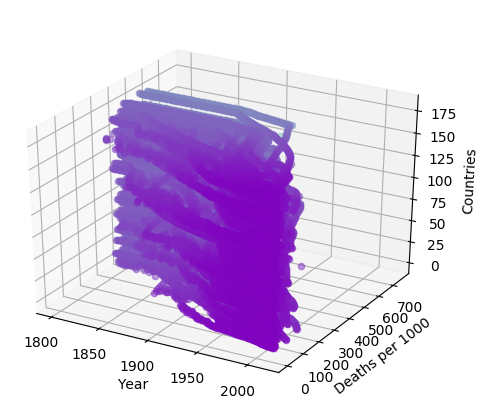
\includegraphics[scale=0.9]{original1.png} \\
		For some countries rates are higher, for some much lower. I have tried to display raw data in 2D plane as well, the result is following:\\
		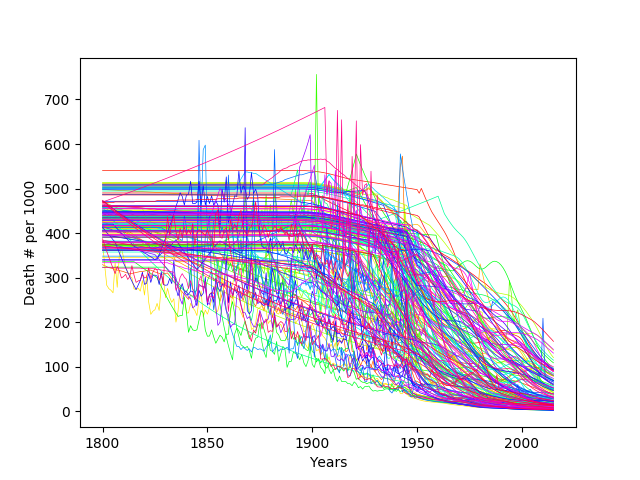
\includegraphics[scale=0.75]{data.png} \\
		We can clearly see here as well, that pretty much for all countries death rate per 1000 people decreases over time. Some countries have too smooth lines, some have picks in data. Anyway, these plots prove that having that many dimensions would make it really hard to analyze the data in general. \\
		
			After parsing data into matrix from the given file, I've got:
		\begin{itemize}
		\item \(X = m \times n\) matrix, where \(m=180\) and \(n = 216\). 
		\item Number of features or dimensions \(d=216\). 
		\item Number of data-points  \(t=180\), where data-points are \(x^0....x^t\), each has dimension \(d\). \\
		\end{itemize}
	{\bf \item Part 1.} Principal Components Analysis (PCA). \\
	
	There are two ways to do dimensionality reduction in ML, feature selection and feature extraction. The PCA is the best known and the most widely used  feature extraction method.  As in all projection methods, in PCA we are interested in finding mapping from the original inputs in the original {\it d}-dimensional space to a new \((k < d)\)-dimensional space, with minimum loss of information. \\ 
	PCA  is an unsupervised method because it does not use the output information and  the criterion that we want to maximize is the variance. In PCA analysis we calculate projection of \(x\) on the direction \(w\): \(z=w^Tx\). And principle component is such \(w\)  where sample is most spread out after projection on it, and difference in samples becomes more apparent.\\
	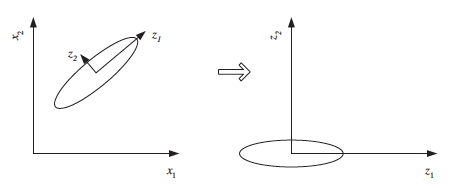
\includegraphics[scale=0.9]{1.png} \\
	In our project, we used singular value decomposition(SVD) method to factor data matrix. The goal of factor analysis is to characterize the dependency among the observed variables by means of a smaller number of factors. Basically, we want to take a set of 180 countries and see if we can do something such that we can group them into smaller subsets with similar characteristics, basically reducing number of dimensions this way. \\
	In SVD method, we decompose data matrix into 3 components:
	\begin{center} \(X = USV^T\), \end{center}
	where \(S\) is a diagonal matrix of singular values in a sorted order, and columns of \(US\) give as principle components. \(V\) columns contain principal directions or projection. Singular values are related to eigenvalues \( \lambda_i \) that show variances of the respective principle components: \( \lambda_i = s_i^2 / (n-1) \). So, the portion of variance covered by first k singular values may be calculated using following formula: \\
	 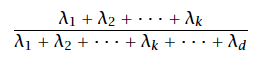
\includegraphics[scale=0.65]{4.png} \\
	After decomposing  \(X\) matrix into 3 matrices I was able to build following plots:\\
	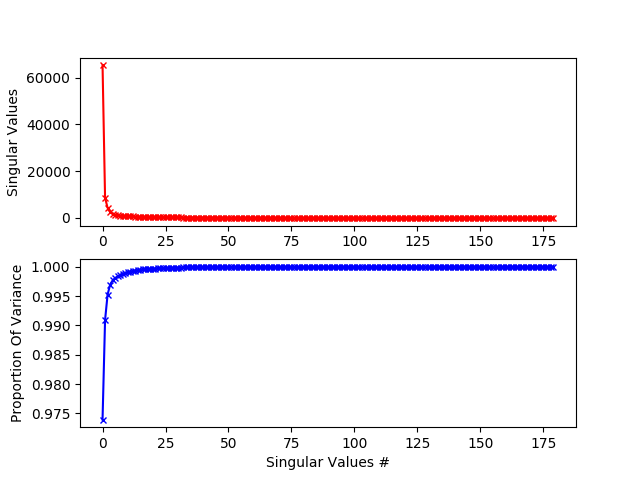
\includegraphics[scale=0.95]{scree.png} \\

	From this picture we can tell that the most significant information is stored now within the first few components. Because we have 180 singular values, it's a bit hard to see how many of those actually matter. I've reduced my picture to only first 25 singular values to see it better:\\
	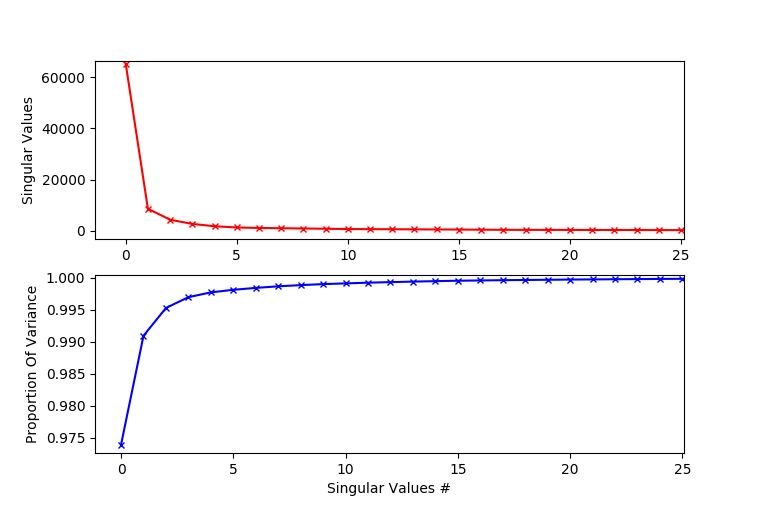
\includegraphics[scale=0.8]{kpcs.png} \\
	
	And what we see is that {\bf 99\%} variance is covered by using first 2 singular values, and thus first 2 principle components are the most valuable. \\
	
	In this project, we had to write a function to reduce data matrix to first {\it k} principle components. And that can be done by multiplying original data matrix by reduced {\it V} vector, such that {\it V} has {\it k} columns for {\it k} principle components:\\
	 \begin{center} \(Z = X V[:k]\), \end{center}
	 After calculating matrix for first 2 principle components I got the following scatter plot for those two components:\\
	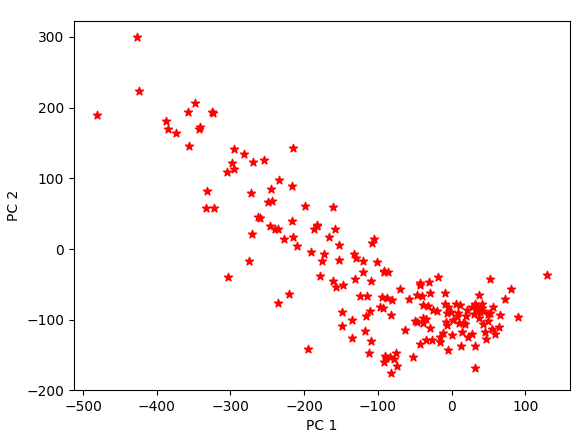
\includegraphics[scale=1]{scatter_pcs1.png} \\
	
	As we can clearly see, reducing number of dimensions from 216 to 2 made its difference. Data is much easier to see. But because there are no labels, we can't really tell anything. Let me add some label. I know it won't look pretty due to plot format and document size but it will show overall picture:\\
	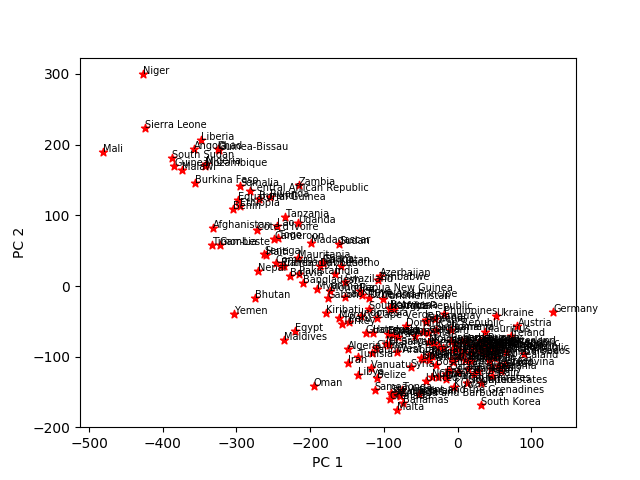
\includegraphics[scale=1.0]{scatter_pcs.png} \\
	
	I also tried to zoom that black spot to see clearly what countries went there. And in the zoomed clusters below it will be possible to see that countries in that cluster are mostly European or the ones with pretty developed infrastructure. At the top of scatter we may see less developed countries with probably higher death rates. \\ 
	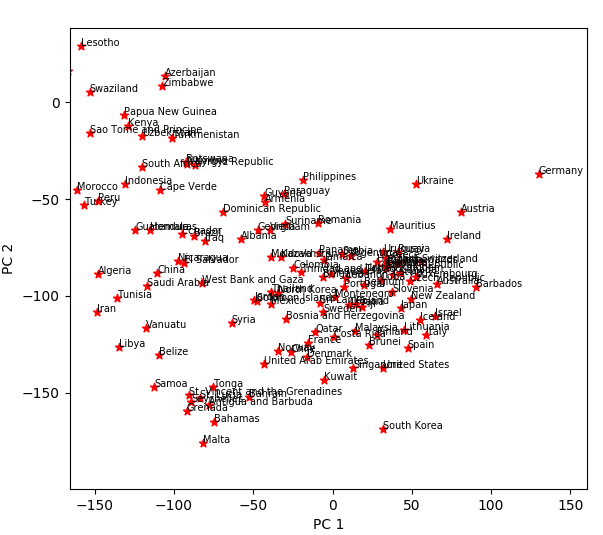
\includegraphics[scale=0.85]{figure_2.png} \\
	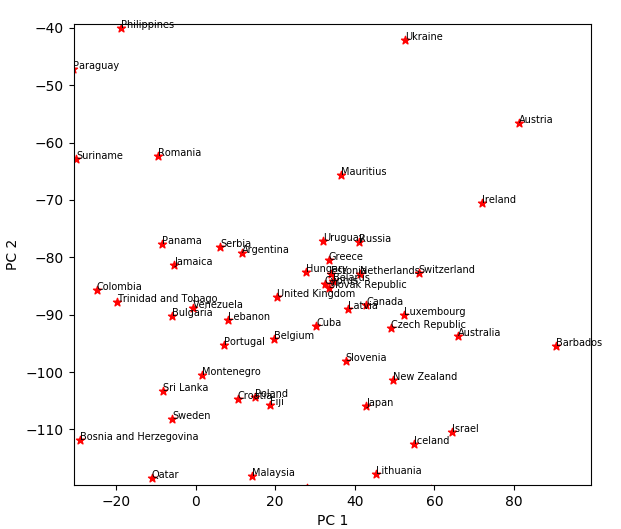
\includegraphics[scale=0.85]{figure_3.png} \\
	
	Now lets move into the second part of project to observe how we can group those counties by groups.
	{\bf \item Part 2.} K-mean clustering. \\
	
	As I stated before, clustering is important when there can be several groups of data in one large data set. So the goal here is to map from a continuous space into discrete and this process is  called  a vector quantization. So, for example if we have a set \(X = \{x^t\}_{t=1}^N \) and k reference vectors \( m_j, j=1,...k \), we want to group all \(x^t \) in k groups/clusters where in each group all \(x^t \) data-points are the most similar with their corresponding \(m_j\) vector.\\ 
	 In a k-mean clustering, such similarity will be calculated using Euclidean distance between two arrays. Initial \(m_i\) will be initialized randomly to data-points from \(X\). Then at each next iteration we use following equation to find out cluster labels for data-points:\\
	 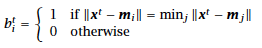
\includegraphics[scale=0.83]{2.png} \\
	 After that we set a new reference vector to means of all those data-points for each cluster.\\
	  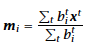
\includegraphics[scale=0.83]{3.png} \\
	  Here is the algorithm outline from the book:\\
	  
	   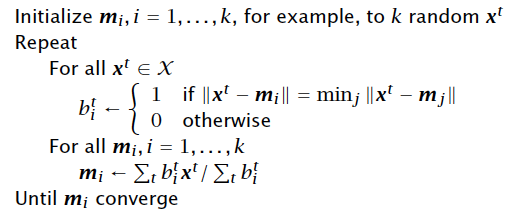
\includegraphics[scale=0.55]{5.png} \\
	  
	  I've structured my program such that when cluster had no values assigned, to avoid undefined mean values I was assigning random data point to it. 
	  
	  I've clustered 3 types of data in my experiment: raw, data that is represented by 2 principle values, and data that is represented by all principle values. For each of those runs I've tried 2 - 7 clusters. I've calculated the Dunn Index for each run, where Dunn index is a metric to judge a clustering algorithm. A higher Dunn index means better clustering and better clustering means that clusters are compact and well-separated from other clusters. To calculate Dunn index we take a ration of minimal inter-cluster distance and maximal intra-cluster distance. For intra-cluster distances I calculated Euclidean distance between all pairs of points in each cluster, chose the maximum. For inter-cluster one, I calculated the distance between means of two clusters: \\
	   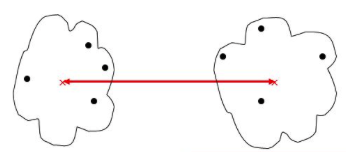
\includegraphics[scale=0.65]{7.png} \\
	   
	    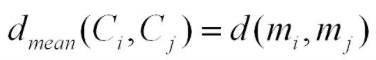
\includegraphics[scale=0.40]{9.png} \\
	    
	  I didn't report inter- and intra- distances themselves, just Dunn index for all runs. Lets look at some results I've got.\\
	  \begin{enumerate}[label=\arabic*.]
		{\bf \item Raw data.}\\
		
		Clearly we can see separation in a data set. But more clusters we have, less it becomes visible what countries should be grouped together. For 2 clusters, a plot somewhat makes sense, since we looked at labels previously and I stated that more developed countries were at the bottom of scatter, and less developed at the top. The bounds for clusters are not very clear.\\
		When we look at the result we 7 clusters it is hard to say if yellow and orange values mapped to the same things. But clearly Bottom 3-4 clusters literally overlap 85\%. That gives us no value.\\\\
		
		
		 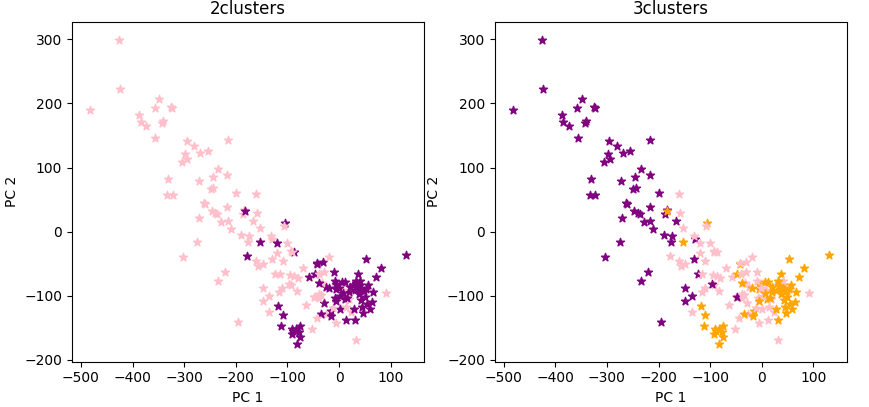
\includegraphics[scale=0.71]{clusters_raw1.png} \\
		  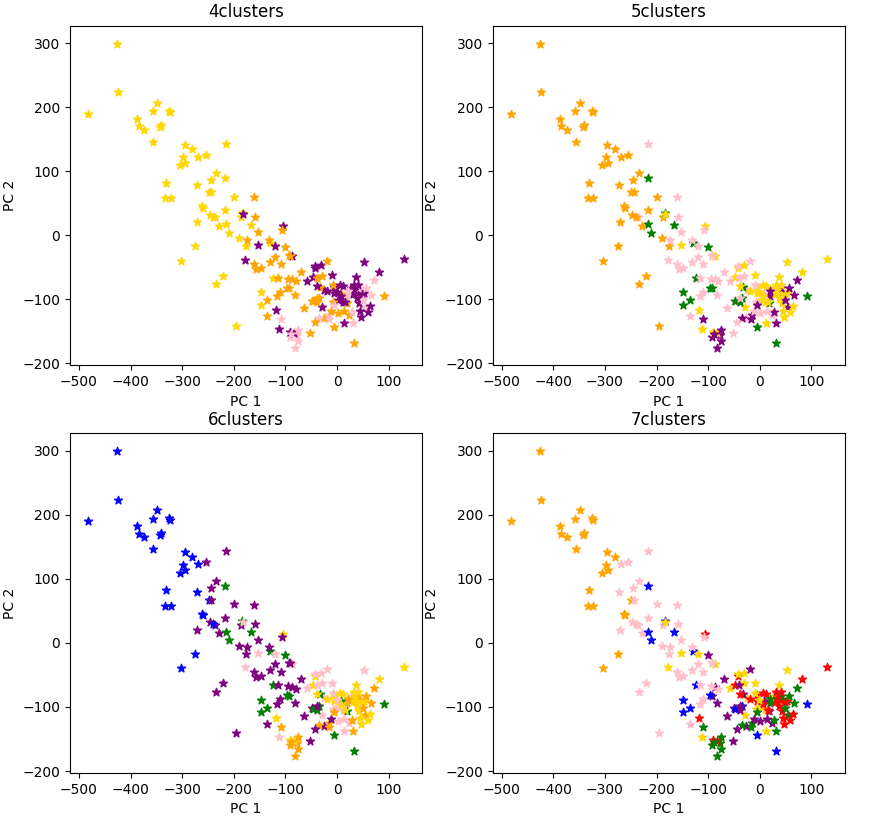
\includegraphics[scale=0.71]{clusters_raw.png} \\
		Lets look at Dunn index and number of iteration before conversion. Here are the results:\\ 
		 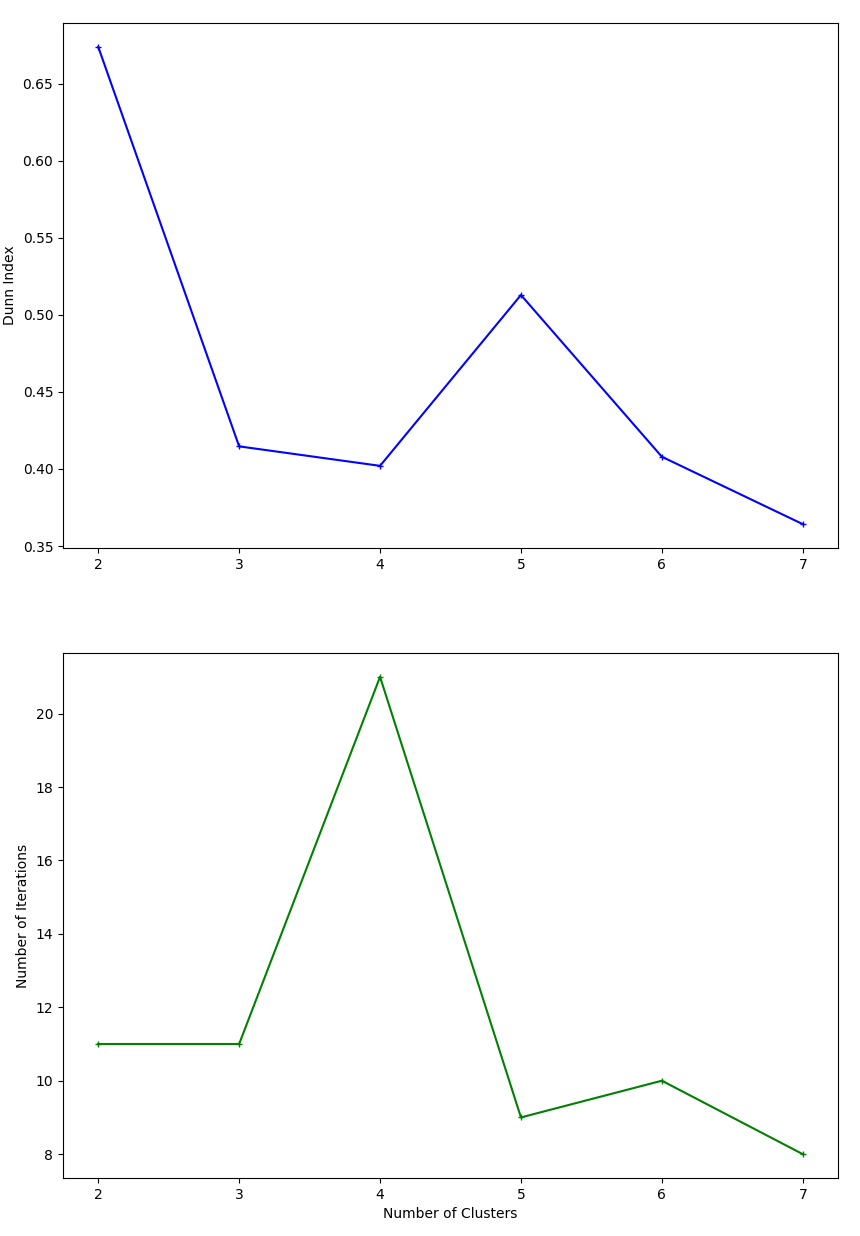
\includegraphics[scale=0.55]{dun_raw.png} \\
		So highest index is for 2 clusters as expected. We have a spike with 5 clusters, but that also might be an error. And clearly with more clusters, index value drops. Number of iterations before convergence doesn't really tell us anything here. \\
		{\bf \item All PCs data.}\\
		
		Results look much better when data is represented in terns of its PCs. All clusters are distinct, they all have approximately the same size and no matter how many clusters we use. I think 6-7 clusters are a bit too much cause we can see how close bottom clusters are, but 2-5 clusters seem to work really nice.\\
		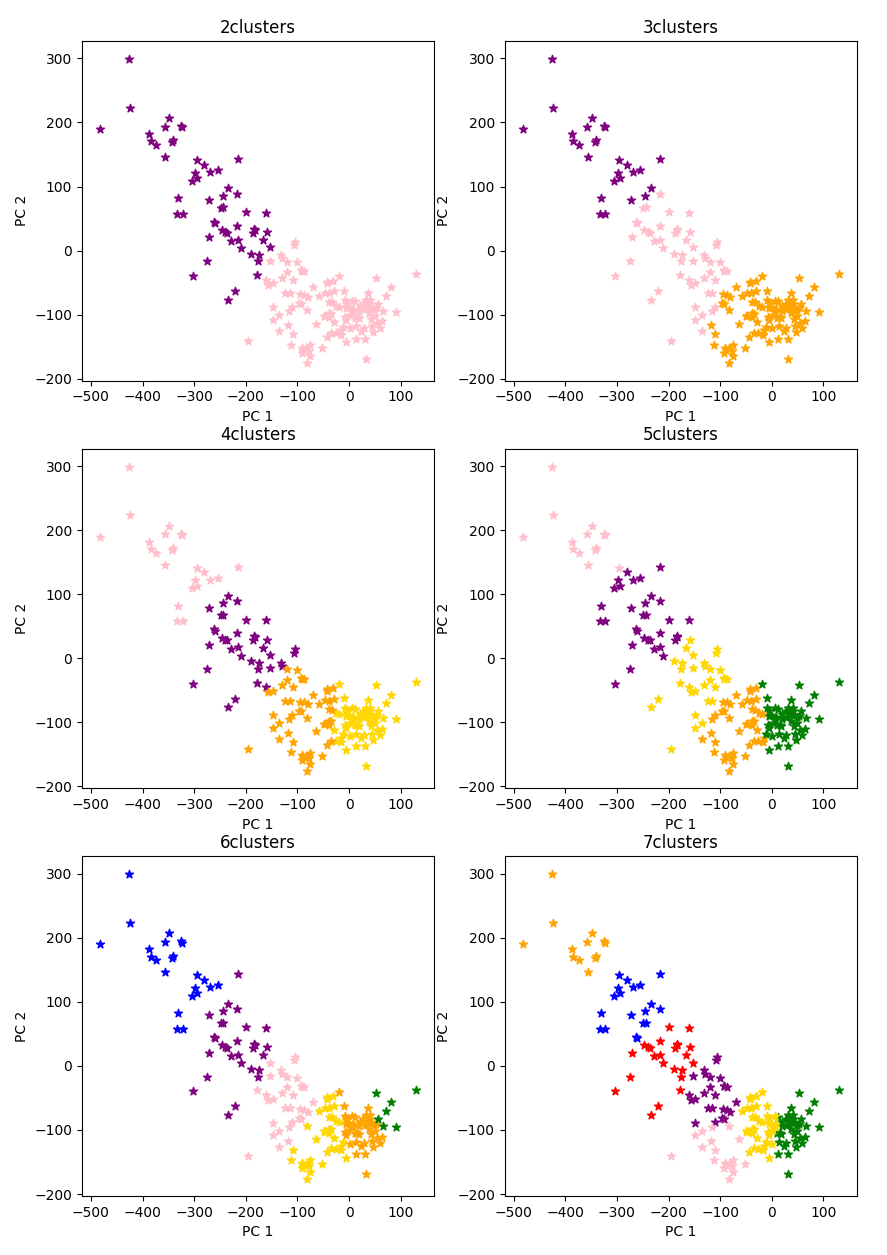
\includegraphics[scale=0.71]{clusters_kpcs.png} \\
		Let's look at Dunn index and number of iterations:\\
		 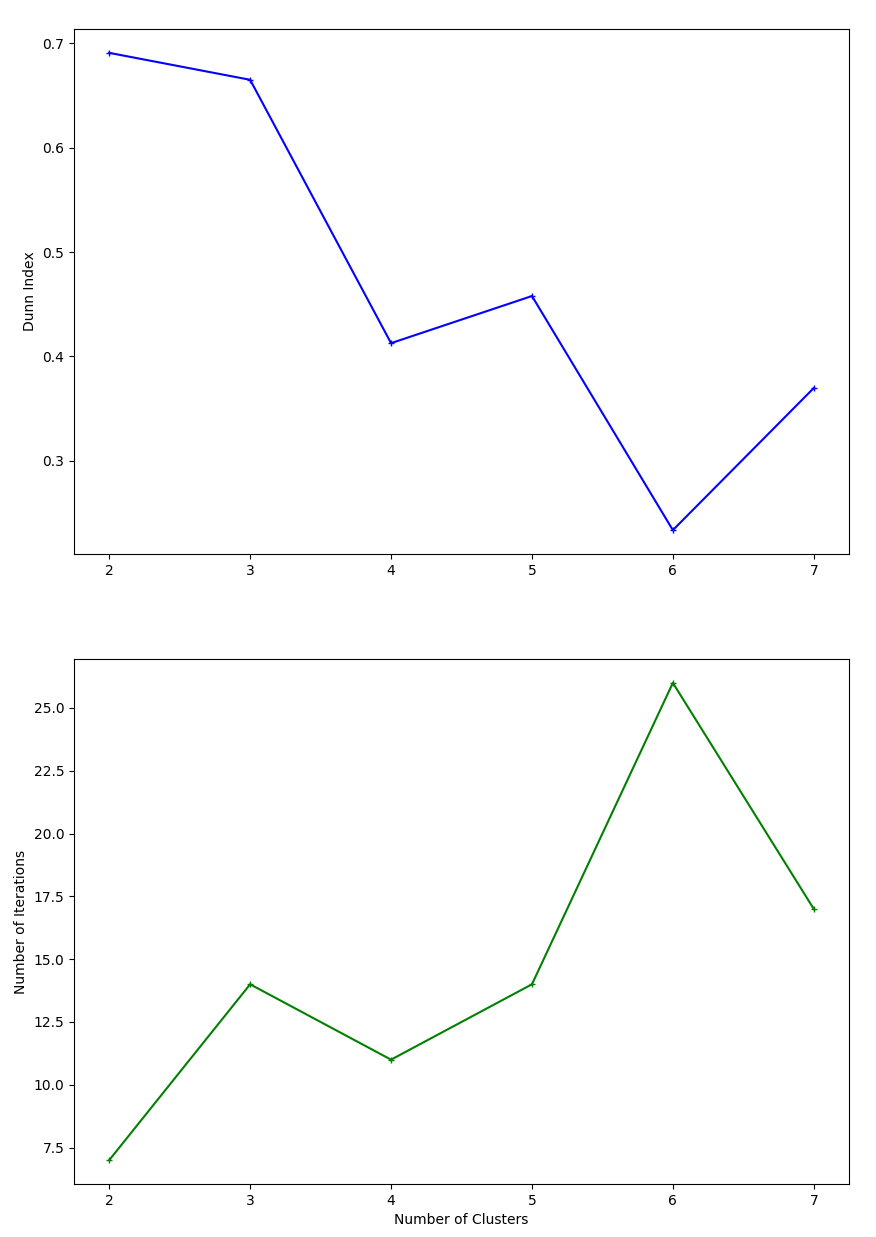
\includegraphics[scale=0.55]{dun_kpcs.png} \\
		 
		 Results seem to be smoother here as well. As I told, best clustering happens with 2-5 clusters. And on average it took longer to converge bigger number of clusters here. But still, it is hard really to tell anything specific about number of iterations for convergence. \\
		 
		 {\bf \item First 2 PCs data.}\\
		 
		 Last test was to run algorithm on data in terms of first 2 PCs. Results are incredibly similar to what we see in previous runs with all PCs but set sizes seem to differ slightly. \\
		 
		 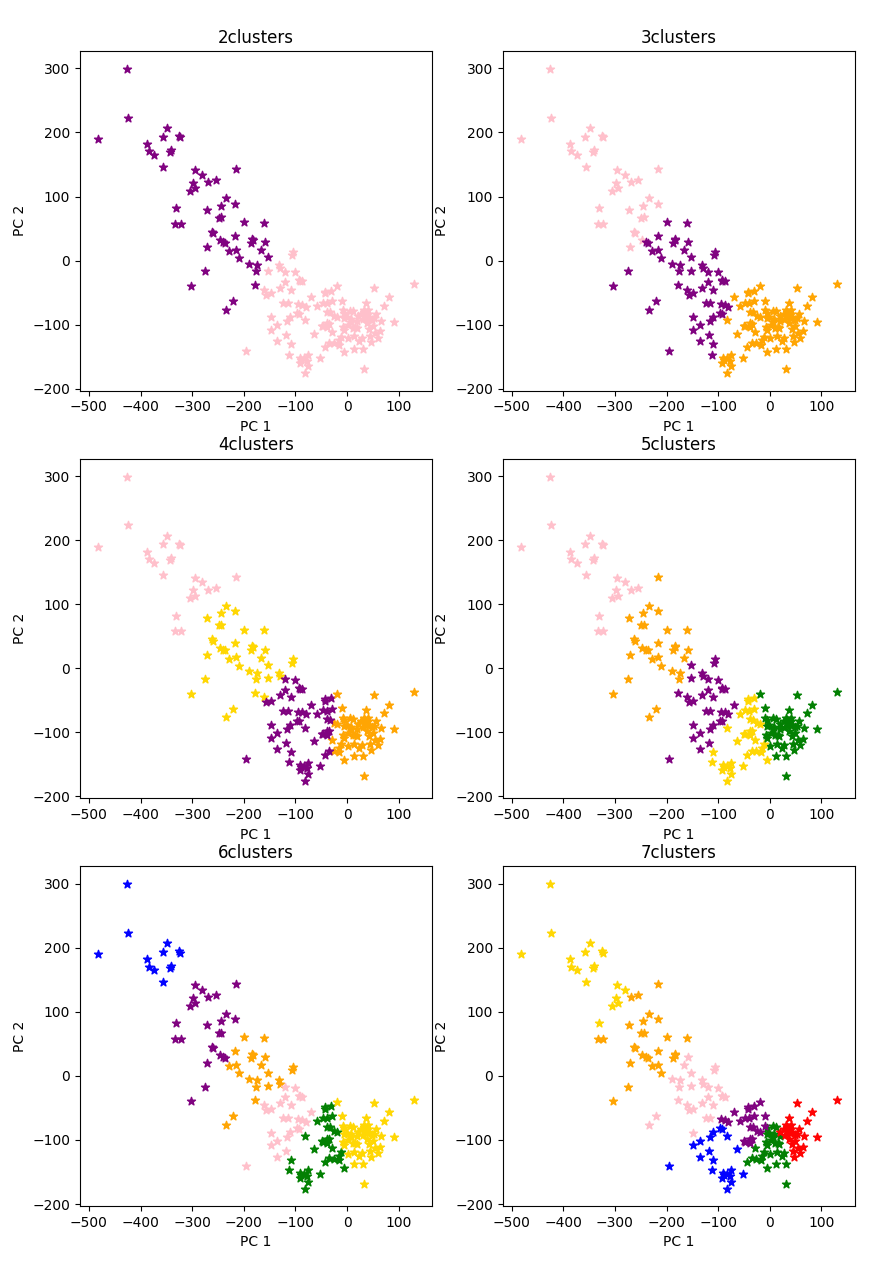
\includegraphics[scale=0.71]{clusters_2pcs.png} \\
		 
		 And the Dunn index is :\\
		  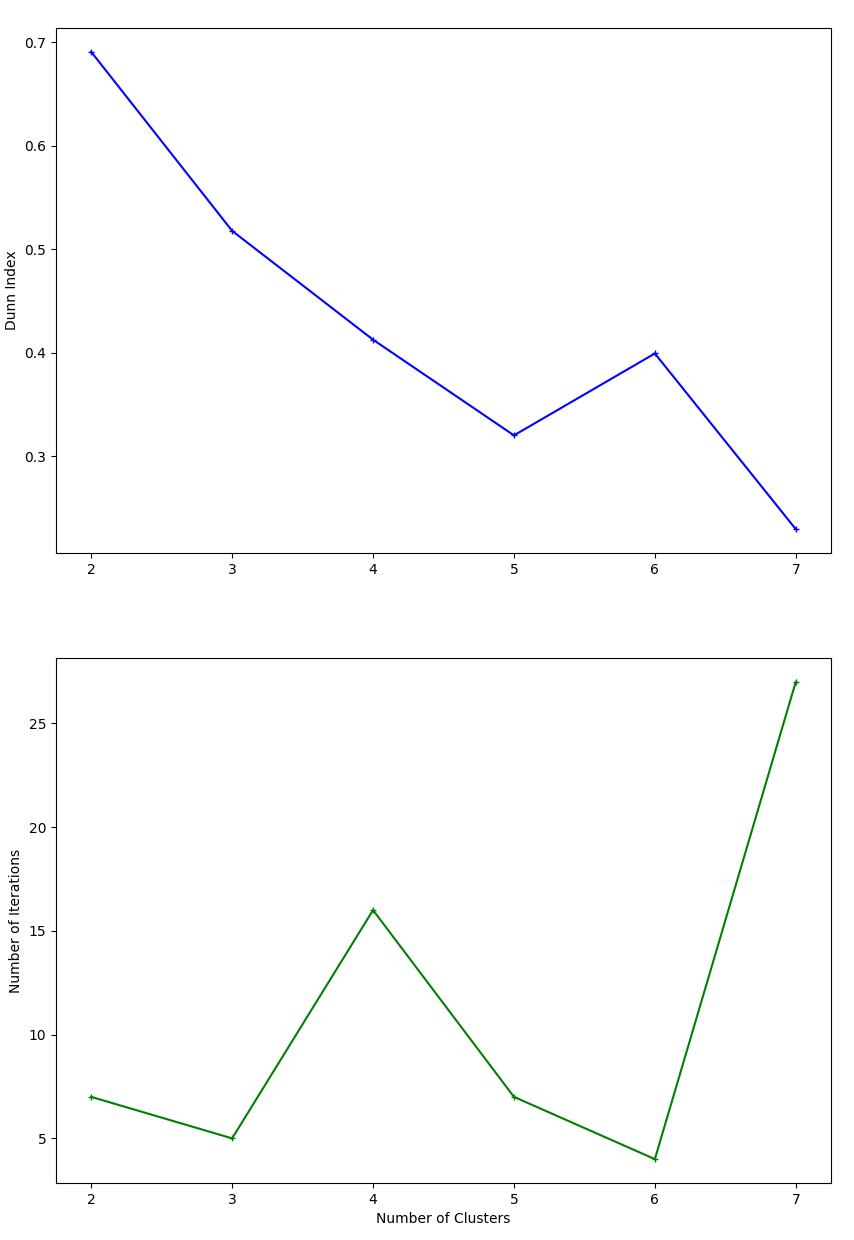
\includegraphics[scale=0.55]{dun_pc2.png} \\
		  
		  The results is much more readable. We can tell for sure that using 2-3 clusters for this data would make the most sense. Clusters in these runs are not only as distinct as in previous experiment, but they also have more even set sizes. It's a bit hard to see but still possible. It makes less sense to use more clusters because the bounds between those clusters start overlapping which makes it hard to decide if a datapoint actually belongs to correct cluster.\\ \\\\\\
	  \end{enumerate}
	 
	  {\bf \item Conclusions.}\\
	  
	  In this project, I was able to see how dimension reduction can be important when trying to explain data set features and just data correlation and variance in general. Looking at the data set at first, I wasn't able to tell how some countries are similar to other in death rates numbers. I could only assume things based on some history and geography knowledge. Representing and visualizing data in terms of first 2 principle components showed how less developed countries shifted to the top and more developed shifted to the bottom of the scatter plot. 
	  With k-means clustering I was able to see how many clusters make sense in categorizing data. We could make up many categories: super-developed, developed, somewhat-developed, not-developed...and etc. based on random parameters, but this algorithm shows that splitting set into 2 - 3 categories works the best. And in fact, when it comes to death rates of children before 5 years old per 1000 people in a country, just development categorization fades away cause there are some other features that may matter that we overlook.
	  
\end{enumerate}
	
	
	
	
	
	
	
\end{document} 